The rectangle $ABCD$ below has dimensions $AB = 12 \sqrt{3}$ and $BC = 13 \sqrt{3}$.  Diagonals $\overline{AC}$ and $\overline{BD}$ intersect at $P$.  If triangle $ABP$ is cut out and removed, edges $\overline{AP}$ and $\overline{BP}$ are joined, and the figure is then creased along segments $\overline{CP}$ and $\overline{DP}$, we obtain a triangular pyramid, all four of whose faces are isosceles triangles.  Find the volume of this pyramid.

\begin{center}
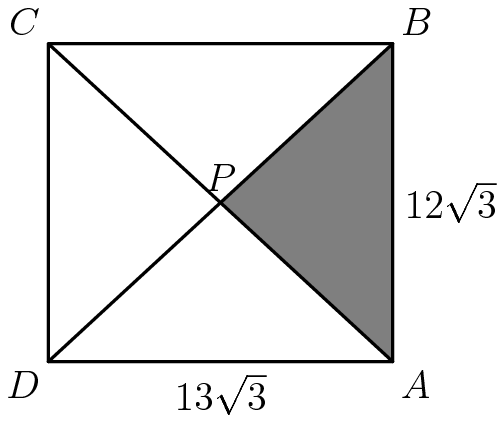
\includegraphics[width = 50.400000000000006mm]{img/fig0.png}
\end{center}